% !TeX root = surprises.tex

\selectlanguage{hebrew}

\chapter{תורת \L{Ramsey}}\label{c.ramsey}

%%%%%%%%%%%%%%%%%%%%%%%%%%%%%%%%%%%%%%%%%%%%%%%%%%%%%%%%%%%
תורת 
\L{Ramsey}
היא תחום בקומבינטוריקה ששואל שאלות מהצורה: מה הגודל המינימלי עבור קבוצה כך שאם מחלקים אותה לתת-קבוצות, לפחות לתת-קבוצה אחת תהיה תכונה מסויימת? קשה להוכיח תוצאות בתורת 
\L{Ramsey}
ויש בעיות פתוחות רבות. בפרק זה נציג מקרים קלים של ארבע בעיות כדי לספק טעימה של תחום מרתק זה: שלשות
\L{Schur}
(סעיף%
~\ref{s.schur})
שהן שלושות של מספרים שלמים כך ש-%
$a+b=c$,
שלשות
\L{Pythagorean}
(סעיף%
~\ref{s.pyth})
שהן שלשות של מספרים שלמים כך ש-%
$a^2+b^2=c^2$,
הבעיה של
\L{van der Waarden}
(סעיף%
~\ref{s.van})
על תכונות של סדרות של מספרים, ותורת
\L{Ramsey}
(סעיף%
~\ref{s.ramsey})
על צביעת גרפים. סעיף%
~\ref{s.bounds}
מראה איך ניתן להשתמש בשיטה הסתברותי כדי למצוא חסם תחתון למספרי
\L{Ramsey}.

הבעיה של שלשות
\L{Pythagorean}
נפתרה לאחרונה בעזרת מחשבים תוך שימוש בשיטה יחסית חדשה הנקראת 
\L{SAT solving}.
עבור קוראים המכירים תחשיב הפסוקים בלוגיקה, סעיף%
~\ref{s.sat}
מביא מבט קצר על השיטה.

סעיף%
~\ref{s.plimpton}
מתאר את שלשות 
\L{Pythagorean}
כפי שהבבלים הכירו לפני כארבעת אלפים שנים.

%%%%%%%%%%%%%%%%%%%%%%%%%%%%%%%%%%%%%%%%%%%%%%%%%%%%%%%%%%%

\section{שלשות \L{Schur}}\label{s.schur}
\index{Schur triples}

\begin{definition}
נתונה חלקה כלשהי של קבוצה של המספרים השלמים:
\[
S(n)=\{1,\ldots,n\}
\]
לשתי תת-קבוצות זרות
$S_1,S_2$,
האם קיימים
$\{a,b,c\}\subseteq S_1$
או
$\{a,b,c\}\subseteq S_2$
(או שניהם) כך ש-%
$a\!<\!b\!<\!c$
ו-%
$a+b=c$?
אם כן, הקבוצה 
$\{a,b,c\}$
נקראת 
\textbf{שלשת \L{Schur}}.
\end{definition}

\textbf{דוגמה}
עבור
$n=8$,
בחלוקה:
\[
S_1 = \{1,2,3,4\},\; S_2 = \{5,6,7,8\}\,,
\label{eq.schur0}
\]
הקבוצה
$S_1$
מכילה את שלשת ה-%
\L{Schur}
$\{1,2,3\}$.
אולם החלוקה:
\[
S'_1 = \{1,2,4,8\},\; S'_2 = \{3,5,6,7\}\,,
\label{eq:schur1}
\]
לא מכילה שלשת
\L{Schur}
כפי שניתן לראות על ידי בדיקת כל השלשות בכל תת-קבוצה.

\begin{theorem}
\textbf{בכל}
חלוקה של
$S(9)=\{1,\ldots,9\}$
לשתי תת-קבוצות זרות, לפחות תת-קבוצה אחת מכילה שלשת
\L{Schur}.
\end{theorem}
כמובן שניתן לבדוק את כל
$2^9=512$
החלוקות של 
$S(9)$
לשתי תת-קבוצות זרות, אבל ננסה למצוא הוכחה תמציתית יותר.

\begin{proof}
ננסה לבנות חלוקה 
\textbf{שלא}
כוללת שלשת
\L{Schur}
ונראה שבגלל אילוצי הבעיה הדבר בלתי אפשרי. תחילה נשים את
$1$
ואת
$3$
ב-%
$S_1$.
$2$
חייב להיות ב-%
$S_2$
כי
$1+2=3$
ואנחנו מנסים לבנות חלוקה שלא כוללת שלשת
\L{Schur}.
באופן דומה, 
$4$
חייב להיות ב-%
$S_2$
כי
$1+3=4$.
נמשיך ונשים את
$6$
ב-%
$S_1$
כי
$2+4=6$
ו-%
$7$
ב-%
$S_2$
כי
$1+6=7$.
אבל
$3+6=9$
ו-%
$2+7=9$,
ולכן
$9$
חייב להופיע גם ב-%
$S_1$
וגם ב-%
$S_2$, 
סתירה. סדרת ההסקות הללו מוצגת בטבלה שלהלן:
\[
\begin{array}{l@{\hspace{2em}}l}
S_1&S_2\\\hline
1,3 & \\
1,3 & 2\\
1,3 & 2,4\\
1,3,6 & 2,4\\
1,3,6 & 2,4,7\\
1,3,6,9 & 2,4,7\\
1,3,6,9 & 2,4,7,9
\end{array}
\]
נחזור לאחור ונחפש חלוקה עם 
$1,3$
בתת-קבוצות שונות. אם נשים עכשיו את 
$5$
ב-%
$S_2$, 
סדרת הסקות שוב מובילה לסתירה כי 
$9$
חייב להופיע בשתי תת-הקבוצות. מומלץ לקורא להצדיק כל אחת מההסקות בטבלה שלהלן:
\[
\begin{array}{l@{\hspace{2em}}l}
S_1&S_2\\\hline
1&3\\
1 & 3,5\\
1,2&3,5\\
1,2,8&3,5\\
1,2,8&3,5,7\\
1,2,8&3,5,7,9\\
1,2,8&3,5,6,7,9\\
1,2,8,9&3,5,6,7,9
\end{array}
\]
שוב נחזור לאחור וננסה לשים את 
$5$
ב-%
$S_1$,
אבל גם זה מוביל לסתירה כפי שאפשר לראות בטבלה שלהלן:
\[
\begin{array}{l@{\hspace{2em}}l}
S_1&S_2\\\hline
1&3\\
1,5& 3\\
1,5&3,4\\
1,5&3,4,6\\
1,2,5&3,4,6\\
1,2,5&3,4,6,7\\
1,2,5,7&3,4,6,7
\end{array}
\]
מכאן שאין חלוקה שלא כוללת שלשת
\L{Schur}.
\end{proof}
\L{Issai Schur}
הוכיח את המשפט:
\begin{theorem}[\L{Schur}]
לכל 
$k\geq 2$
קיים 
$n$
קטן ביותר כך שבכל חלוקה של
$S(n)$
ל-%
$k$
תת-קבוצות זרות לפחות תת-קבוצה אחת תכיל שלשת
\L{Schur}.
\end{theorem}

%%%%%%%%%%%%%%%%%%%%%%%%%%%%%%%%%%%%%%%%%%%%%%%%%%%%%%%%%%%

\section{שלשות \L{Pythagorean}}\label{s.pyth}

\begin{definition}נתונה חלקה כלשהי של קבוצה של המספרים השלמים:
\[
S(n)=\{1,\ldots,n\}
\]
לשתי תת-קבוצות זרות
$S_1,S_2$,
האם קיימים
$\{a,b,c\}\subseteq S_1$
או
$\{a,b,c\}\subseteq S_2$
(או שניהם) כך ש-%
$a\!<\!b\!<\!c$
ו-%
$a^2+b^2=c^2$?
אם כן, הקבוצה 
$\{a,b,c\}$
נקראת 
\textbf{שלשות \L{Pythagorean}}.\index{Pythagorean triples}
\end{definition}

\textbf{דוגמה}
עבור
$n=10$
בחלוקה למספרים זוגיים ואי-זוגיים:
\[
S_1 = \{1,3,5,7,9\},\; S_2=\{2,4,6,8,10\}\,,
\]
אין שלשות
\L{Pythagorean}
ב-%
$S_1$
אבל  
$\{6,8,10\}$
ב-%
$S_2$
היא
שלשות
\L{Pythagorean}
כי
$6^2+8^2=10^2$.


\L{Marijn J.H. Heule}\index{Heule, Marijn J.H.}
ו-%
Oliver Kullmann\index{Kullman, Oliver}
הוכיחו את המשפטים שלהלן. שיטת ההוכחה מתוארת בסעיף%
~\ref{s.sat}.

\begin{theorem}
לכל 
$n\leq 7824$
\textbf{קיימת}
חלוקה של 
$S(n)$
לשתי תת-קבוצות זרות כך
\textbf{שאף אחת מתת-הקבוצות לא כולל}
שלשות
\L{Pythagorean}.
\end{theorem}

\begin{theorem}
לכל 
$n\geq 7825$
\textbf{בכל}
חלוקה של 
$S(n)$
לשתי תת-קבוצות זרות 
\textbf{לפחות תת-קבוצה אחת מכילה}
שלשות
\L{Pythagorean}.
\end{theorem}
אין כל אפשרות לבדוק את כל
$2^{7825}$
החלוקות של
$S(7825)$.
לו יכולנו לבדוק חלוקה אחת כל מיקרושניה, 
$2^{7825}\; \textrm{מיקרושניות}\approx 10^{600}\; \textrm{שנים}$, 
בעוד הגיל הממוצע של היקום הוא רק
$10^{10}$
שנים.

%%%%%%%%%%%%%%%%%%%%%%%%%%%%%%%%%%%%%%%%%%%%%%%%%%%%%%%%%%%

\section{\L{Van der Waerden} הבעיה של}\label{s.van}

נעיין בסדרות של שמונה נקודות צבעוניות באיור%
~\ref{f.vdw1}.
בסדרה הראשונה נקודות אדומות נמצאות במקומות
$(1,2,3)$
ונקודות כחולות במקומות
$(4,5,6)$.
בשני המקרים המקומות מהווים סדרה חשבונית. באופן דומה, בסדרה השניה המקומות של הנקודות האדומות
$(1,3,5)$
מהווים סדרה חשבונית. לעומת זאת, בסדרה השלישית אין קבוצה של שלוש נקודות חד-צבעוניות שמקומותיהן מהווים סדרה חשבונית. המקומות של אף אחת מהשלשות של נקודות אדומות 
$(1,2,5)$, $(1,2,6)$, $(2,5,6)$
לא מהווים סדרה חשבונית וכנ"ל עבור נקודות כחולות.
\begin{figure}[htb]
\begin{center}
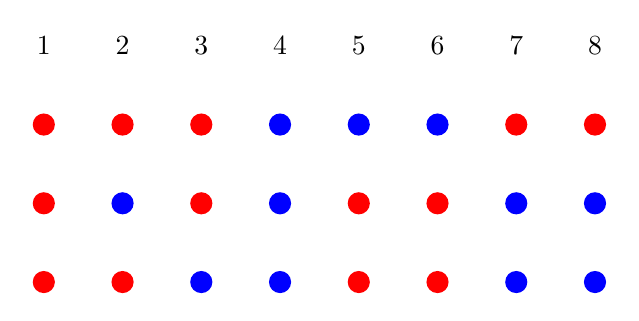
\begin{tikzpicture}
\foreach \x in {1,2,3,4,5,6,7,8} {
  \node at (\x,3) {$\x$};
}
\foreach \x/\col in {1/red,2/red,3/red,4/blue,5/blue,6/blue,7/red,8/red} {
  \fill[\col] (\x,2) circle(4pt);
}
\foreach \x/\col in {1/red,2/blue,3/red,4/blue,5/red,6/red,7/blue,8/blue} {
  \fill[\col] (\x,1) circle(4pt);
}
\foreach \x/\col in {1/red,2/red,3/blue,4/blue,5/red,6/red,7/blue,8/blue} {
  \fill[\col] (\x,0) circle(4pt);
}
\end{tikzpicture}
\end{center}
\caption{בעיית \L{Van der Waerden} עבור שמונה נקודות}\label{f.vdw1}
\end{figure}

עבור תשע נקודות
\textbf{כל}
צביעה
\textbf{חייבת}
להכיל סדרה של שלוש נקודות חד-צבעוניות שמקומותיהן מהווים סדרה חשבונית. למשל, נוסיף נקודה אדומה או נקודה כחולה בסוף הסדרה השלישית באיור%
Fig.~\ref{f.vdw1}
ונקבל את הסדרות בסעיף%
~\ref{f.vdw2}.
בסדרה הראשונה יש נקודות אדומות במקומות
$(1,5,9)$
שהיא סדרה חשבונית, ובסדרה השניה יש נקודות כחולות במקומות 
$(7,8,9)$
שהיא גם סדרה חשבוניות.
\begin{figure}[htb]
\begin{center}
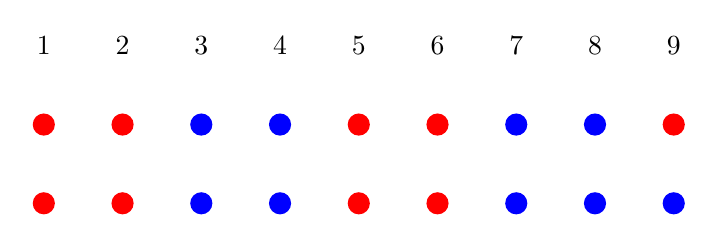
\begin{tikzpicture}
\foreach \x in {1,2,3,4,5,6,7,8,9} {
  \node at (\x,2) {$\x$};
}
\foreach \x/\col in {1/red,2/red,3/blue,4/blue,5/red,6/red,7/blue,8/blue,9/red} {
  \fill[\col] (\x,1) circle(4pt);
}
\foreach \x/\col in {1/red,2/red,3/blue,4/blue,5/red,6/red,7/blue,8/blue,9/blue} {
  \fill[\col] (\x,0) circle(4pt);
}
\end{tikzpicture}
\end{center}
\caption{בעיית \L{Van der Waerden} עבור תשע נקודות}\label{f.vdw2}
\end{figure}

\L{Bartel L. Van der Waerden}
\index{van der Waerden, Bartel L.}
הציג את הבעיה:
\index{van der Waerden's problem}
לכל מספר שלם חיובי
$k$
מה המספר הקטן ביותר 
$n$
כך 
\textbf{שכל}
סדרה של 
$n$
נקודות צבעיניות
\textbf{חייבת להכיל}
סדרה של
$k$
נקודות חד-צבעוניות שמקומותיהן מהווים סדרה חשבונית? עבור
$k=3$
ראינו ש-%
$n=9$.
הוכחת התוצאה הבאה היא קשה הרבה יותר: עבור
$k=4$, $n=35$.

%%%%%%%%%%%%%%%%%%%%%%%%%%%%%%%%%%%%%%%%%%%%%%%%%%%%%%%%%%%

\section{משפט \L{Ramsey}}\label{s.ramsey}

נצבע עם שני צבעים את הקשתות של 
$K_5$, 
הגרף השלם על 
$5$
צמתים
(\ref{f.ramsey5}).
אין תת-גרפים חד-צבעוניים 
$K_3$
(משולשים) בגרף.
~\ref{f.ramsey6}
מראה צביעה אחת של 
$K_6$
וניתן לראות שיש משולשים חד-צבעוניים 
$\triangle ACE$
ו-%
$\triangle BDF$.
סעיף זה נוכיח מקרה פשוט של משפטו של
\L{Frank P. Ramsey}\index{Ramsey, Frank P.}
על קיומן של תת-קבוצות עם תכונה מסויימת.
\begin{figure}[ht]
\selectlanguage{hebrew}
\subcaptionbox{צביעה של $K_5$ עם שני צבעים \label{f.ramsey5}}%
[.45\textwidth]
{
\centering
\begin{tikzpicture}
\node (pentagon) [minimum size=5cm,regular polygon,regular polygon sides=5] at (0,0) {};
\draw[red]  (pentagon.corner 1) node[black,above] {$A$} -- (pentagon.corner 2);
\draw[red]  (pentagon.corner 2) node[black,left] {$B$} -- (pentagon.corner 3);
\draw[red]  (pentagon.corner 3) node[black,left] {$C$} -- (pentagon.corner 4);
\draw[red]  (pentagon.corner 4) node[black,right] {$D$} -- (pentagon.corner 5);
\draw[red]  (pentagon.corner 5) node[black,right] {$E$} -- (pentagon.corner 1);
\draw[dashed,blue] (pentagon.corner 1) -- (pentagon.corner 3);
\draw[dashed,blue] (pentagon.corner 1) -- (pentagon.corner 4);
\draw[dashed,blue] (pentagon.corner 2) -- (pentagon.corner 4);
\draw[dashed,blue] (pentagon.corner 2) -- (pentagon.corner 5);
\draw[dashed,blue] (pentagon.corner 3) -- (pentagon.corner 5);
\end{tikzpicture}
}
\hspace{3em}
\subcaptionbox{צביעה של $K_6$ עם שני צבעים \label{f.ramsey6}}
[.45\textwidth]
{
\centering
\begin{tikzpicture}
\node (hexagon) [minimum size=5cm,regular polygon,regular polygon sides=6] at (0,0) {};
\draw[red]  (hexagon.corner 1) node[black,above] {$A$} -- (hexagon.corner 2);
\draw[red]  (hexagon.corner 2) node[black,above] {$B$} -- (hexagon.corner 3);
\draw[red]  (hexagon.corner 3) node[black,left] {$C$} -- (hexagon.corner 4);
\draw[red]  (hexagon.corner 4) node[black,left] {$D$} -- (hexagon.corner 5);
\draw[red]  (hexagon.corner 5) node[black,right] {$E$} -- (hexagon.corner 6);
\draw[red]  (hexagon.corner 6) node[black,right] {$F$} -- (hexagon.corner 1);
\draw[dashed,blue] (hexagon.corner 1) -- (hexagon.corner 3);
\draw[dashed,blue] (hexagon.corner 1) -- (hexagon.corner 4);
\draw[dashed,blue] (hexagon.corner 1) -- (hexagon.corner 5);
\draw[dashed,blue] (hexagon.corner 2) -- (hexagon.corner 4);
\draw[dashed,blue] (hexagon.corner 2) -- (hexagon.corner 5);
\draw[dashed,blue] (hexagon.corner 2) -- (hexagon.corner 6);
\draw[dashed,blue] (hexagon.corner 3) -- (hexagon.corner 5);
\draw[dashed,blue] (hexagon.corner 3) -- (hexagon.corner 6);
\draw[dashed,blue] (hexagon.corner 4) -- (hexagon.corner 6);
\end{tikzpicture}
}
\end{figure}


\begin{definition}
$\quad R(k)$,
\textbf{מספר
\L{Ramsey}}
עבור 
$k$,
הוא המשר שלם הקטן ביותר 
$n$
כך 
\textbf{שבכל}
צביעה עם שני צבעים של
$K_{n}$,
הגרף השלם מעל 
$n$
צמתים, קיימ תת-גרף שלם 
$K_k$
שהוא חד-ציבעונית.
\end{definition}
\index{Ramsey's theorem}
\begin{theorem}[\L{Ramsey}]
$\quad R(3)=6$.\label{thm.ramsey}
\end{theorem}

\begin{proof}\index{Ramsey's theorem!proof that $R(3)=6$}
איור%
~\ref{f.ramsey5}
מראה ש-%
$R(3)>5$.
כדי להראות ש-%
$R(3)\leq 6$
ניקח צומת שרירותי 
$v$
ב-%
$K_6$.
$v$
מחובר לחמשת הצמתים האחרים וכאשר הקשתות צבועות עם שני צבעים, לפחות שלוש קשתות חד-צבעוניות יהיו מחוברות ל-%
$v$. 

באיור%
~\ref{f.ramsey4a}, $\overline{AB}, \overline{AC}, \overline{AE}$ 
צבועים באדום. הגרף שלם ולכן כל הצמתים מחוברים, כך שאם אחת מהקשתות 
$\overline{BC}$, $\overline{BE}$, $\overline{CE}$
צבועה באדום, נניח
$\overline{BE}$,
משולש אדום נוצר. אחרת כל שלושת הקשתות צבועות בכחול והם מייצרים משולש כחות (איור%
~\ref{f.ramsey4b}).
\end{proof}

ניתן להכליל את המשפט לכל מספר של צבעים וכן לתת-גרפים שאינם בגודל אחיד. 
$R(r,b,g)$
הוא הגרף השלם הקטן ביותר כך שבכל צביעה עם שלושה צבעים חייב להיות תת-גרפים שלמים עם 
$r$
קשתות אדומות, 
$b$
כחולות ו-%
$g$
ירוקות.

\begin{figure}[t]
\centering
\selectlanguage{hebrew}
\subcaptionbox{%
צומת אחד של
$K_6$\label{f.ramsey4a}}
[.45\textwidth]
{
\centering
\begin{tikzpicture}
\node (hexagon) [minimum size=5cm,regular polygon,regular polygon sides=6] at (0,0) {};
\draw[red]  (hexagon.corner 1) node[black,above] {$A$} -- (hexagon.corner 2) node[black,above] {$B$};
\draw[blue,dashed]  (hexagon.corner 1) -- (hexagon.corner 6) node[black,right] {$F$};
\draw[red] (hexagon.corner 1) -- (hexagon.corner 3) node[black,below] {$C$};
\draw[blue,dashed] (hexagon.corner 1) -- (hexagon.corner 4) node[black,right] {$D$};
\draw[red] (hexagon.corner 1) -- (hexagon.corner 5) node[black,right] {$E$};
\end{tikzpicture}
}
\hspace{3em}
\subcaptionbox{%
משולשים חד-צבעוניים ב-%
$K_6$\label{f.ramsey4b}}
[.45\textwidth]
{
\centering
\begin{tikzpicture}
\node (hexagon) [minimum size=5cm,regular polygon,regular polygon sides=6] at (0,0) {};
\draw[very thick,red]  (hexagon.corner 1) node[black,above] {$A$} -- (hexagon.corner 2) node[black,above] {$B$};
\draw[blue,dashed]  (hexagon.corner 1) -- (hexagon.corner 6) node[black,right] {$F$};
\draw[red] (hexagon.corner 1) -- (hexagon.corner 3) node[black,below] {$C$};
\draw[blue,dashed] (hexagon.corner 1) -- (hexagon.corner 4) node[black,right] {$D$};
\draw[very thick,red] (hexagon.corner 1) -- (hexagon.corner 5) node[black,right] {$E$};
\draw[very thick,red] (hexagon.corner 2) -- (hexagon.corner 5);
\draw[very thick,blue,dashed] (hexagon.corner 2) -- (hexagon.corner 3);
\draw[very thick,blue,dashed] ($(hexagon.corner 2)+(-2pt,0)$) -- ($(hexagon.corner 5)+(-2pt,0)$);
\draw[very thick,blue,dashed] (hexagon.corner 5) -- (hexagon.corner 3);
\end{tikzpicture}
}
\end{figure}

%%%%%%%%%%%%%%%%%%%%%%%%%%%%%%%%%%%%%%%%%%%%%%%%%%%%%%%%%%%

\section{The Probabilistic Method}\label{s.bounds}

רק שני מספרי 
\L{Ramsey}
לא טרביאליים ידועים:
$R(3)=6$
ו-%
$R(4)=18$.
ב-%
$1947$
\L{Paul Erd\H{o}s}\index{Paul Erdos@Paul Erd\H{o}s}
פיתח את 
\textbf{השיטה ההסתברותית}
\index{Probabilistic method} 
והשתמש בה כדי להראות חסמים עליונים ותחתונים עבור
$R(k)$.\index{Ramsey's theorem!lower bound}
מחקרים נוספים שיפרו את החסמים אבל נושא זה הוא עדיין פתוח למחקרים נוספים כי החסמים אינם הדוקים. למשל, הוכח ש-%
$43\leq R(5) \leq 48$
ו-%
$798\leq R(10)\leq 23556$.
בסעיף זה נשתמש בהסתברות פשוטה כדי להוכיח חסם תחתון עבור 
$R(k)$.

כדי להראות שקיים איבר בקבוצה 
$S$
עם תכונה 
$A$,
מספיק להוכיח שההסתברות שלאיבר
\textbf{אקראי}
של התכונה 
$A$
היא גדול מאפס. חשוב להבין שהשיטה היא 
\textbf{לא בונה}:
היא רק מוכיחה שקיים איבר העונה על הדרישה אבל לא בונה איבר. למרות שידועה לנו מ-%

~\ref{thm.ramsey}
ש-%
$R(3)=6$,
נשתמש בשיטה ההסתברותית כדי להוכיח חסם תחתון עבור
$R(3)$.\index{Ramsey's theorem!lower bound for}

\begin{theorem}[\L{Erd\H{o}s}]
$\quad R(3) > 4$.
\end{theorem}
\begin{proof}
נתונה צביעה 
\textbf{אקראית}
של
$K_n$
בשני צבעים, נעיין בתת-גרף שרירותי
$K_3$,
כלומר, משולש שרירותי עם
$\dischoose{3}{2}=3$
צלעות. ההסתברות שכל הצלעות צבועים באדום היא
$2^{-3}$
כמו גם ההסתברות שכל הצלעות צבעים בכחול. לכן ההסתברות שהמשולש הוא חד-צבעונית היא
$2^{-3}+2^{-3}=2^{-2}=1/4$.
מספר המשולשים ב-%
$K_n$
הוא
$\dischoose{n}{3}$, 
ולכן,
$P(n,3)$,
ההסתברות שקיים משולש חד-צבעונית בצביעה אקראית של 
$K_n$,
היא:
\[
P(n,3)=\dischoose{n}{3}\cdot \frac{1}{4}\,.
\]
אם
$P(n,3)<1$
אזי המשלים שלה 
$\overline{P}(n,3)=1-P$
גדול מ-%
$0$,
כלומר, ההסתברות שצביעה אקראית של 
$K_n$
\textbf{לא מכילה}
משולש חד-צבעונית גדולה מאפס וצביעה אחת כזאת חייבת להתקיים.

הטבלה שלהלן מראה
$\overline{P}(n,3)$
עבור מספר ערכים של
$n$,
ולכל אחד האם הערך של
$\overline{P}(n,3)$
מוכיח שקיים צביעה ללא משולש חד-צבעונית:
\[
\renewcommand*{\arraystretch}{1.1}
\begin{array}{r@{\hspace{5mm}}r@{\hspace{5mm}}r}
\hline
\noalign{\smallskip}
n & \overline{P}(n,3) & \textrm{קיימת}\\
\noalign{\smallskip}\hline\noalign{\smallskip}
3 & 3/4 & \textrm{כן} \\
4 & 5/6 & \textrm{כן}\\
5 & -3/7 & \textrm{--}\\
\noalign{\smallskip}
 \hline
 \end{array}
\]
\end{proof}

במבט ראשון התוצאה מוזרה כי איור%
~\ref{f.ramsey5}
מראה שיש צביעה של
$K_5$
ללא משולש חד-צבעונית. אולם, הקריטריון ההסתברותי מספיק ולא הכרחי. מדובר בחסם תחתון שמוכיח ש-%
$R(n)>4$,
טענה נכונה כי ראינו במשפט%
~\ref{thm.ramsey}
ש-%
$R(n)=6$.

אותה הוכחה תקפה עבור
$k$
שרירותי ולכן ההסתברות שקיימת צביעה של 
$K_n$
ללא גרף שלם 
$K_k$
חד-צבעוני היא:
\[
P(n,k)=\dischoose{n}{k}\cdot 2\cdot 2^{-{k \choose 2}}\,.
\]
For $k=4$:
\begin{eqnarray*}
\overline{P}(n,4)&=&1-\dischoose{n}{4}\cdot 2^{-5}=\left.\left(32-\dischoose{n}{4}\right)\right/32\\
\overline{P}(6,4)&=&(32-15)/32=17/32\\
\overline{P}(7,4)&=&(32-35)/32=-3/32\,.
\end{eqnarray*}
מכאן ש-%
$R(4)>6$
שהוא קטן הרבה יותר מהערך הידוע
$R(4)=18$.

%%%%%%%%%%%%%%%%%%%%%%%%%%%%%%%%%%%%%%%%%%%%%%%%%%%%%%%%%%%

\section{\L{SAT Solving}}\label{s.sat}

\L{SAT Solving}
היא שיטה לפתרון בעיות בה מקדדים את הבעיה בנוסחה בתחשיב בפסוקים ואז משתמשים בתכנית מחשב כדי לבדוק את ערך האמת של הנוסחה. התקדמות באלגוריתמים ובמימושם מאפשרות פתרונות מעשיים למגוון בעיות. נביא סקירה של 
\L{SAT Solving}
ונסביר איך להשתמש בה כדי לפתור את הבעיות המתמטיות שתיארנו בפרק זה. אנו מניחים שלקורא ידע בסיסי בתחשיב הפסוקים כדי שמוצג בהגדרה%
~\ref{def.sat}.\index{Propositional logic}

\subsection{תחשיב הפסוקים ובעיית \L{SAT}}

\begin{definition}\label{def.sat}
\mbox{}\\
\vspace{-4ex}
\begin{itemize}
\item
\textbf{נוסחה}
\L{(formula)}
מורכבת מ-%
\textbf{נוסחאות אטומיות}
\L{(atomic formula)}
או
\textbf{אטומים}
\L{(atom)}
בחוברים ב-%
\textbf{אופרטורים}
\L{(operators)}:
$\vee$ (\L{disjunction}, "או"),
$\wedge$ (\L{conjunction}, "וגם"),
$\neg$ (\L{negation}, "לא").

\item
נוסחה מקבלת משמעות על ידי 
\textbf{פירוש}
\L{(interperation)}
שהוא השמה של
$T$
או
$F$
לכן אטום. חישוב נוסחה בפירוש נותן 
\textbf{ערך אמת}
\L{(truth value)}
$T$
או
$F$. 

\item
נוסחה היא
\textbf{ספיקה}
\L{(satisfiable)}
אם ורק אם קיים פירוש שבו ערך האמת שלה הוא
$T$.
אחרת, הנוסחה היא
\textbf{בלתי ספיקה}
\L{(unsatisfiable)}.

\item
נוסחה היא בצורת
\L{CNF}
(קיצור של
\L{conjunctive normal form})
אם ורק אם היא מורכת מתת-נוסחאות המחוברות ב-"וגם", כאשר כל תת-נוסחה מורכבת מ-"ליטרלים" (אטומים או שלילה של אטומים) מחוברים ב-"או".
\end{itemize}
\end{definition}

נוסחה זו היא בצורת
\L{CNF}:
\[
(\neg p \vee q \vee \neg \,r) \;\wedge\; (\neg p \vee r)
\;\wedge\; (\neg \,r)\;\wedge\;(p \vee q \vee \neg \,r)\,.
\]

בעיית
\L{SAT}
היא להכריע אם נוסחה נתונה ב-%
\L{CNF}
ספיקה או לא. 
\L{SAT solver}\index{SAT solver}
היא תכנית מחשב לפתור בעיות
\L{CNF}.
רוב ה-%
\L{CNF}
מבוססות על אלגוריתם
\L{DPLL}
שפותח כבר שנות ה-%
$1960$,
אבל התקדמות מודרניות הביאו לשיפורים מאוד משמעותיים באלגוריתם. בעקבות פיתוח מימושים יעילים של האלגוריתמים הללו 
\L{SAT solver}
הפכו להיות כלים חשובים לפתרון של בעיות בהרבה שטחים כולל במתמטיקה.

\subsection{שלשות \L{Schur}}\index{Schur triples}

נקדד את בעיית שלושות
\L{Schur}
עבור 
$S(8)$
כנוסחה ב-%
\L{CNF}.
הנוסחה תהיה ספיקה אם ורק אם קיימת חלוקה של 
$S$
לשתי תת-קבוצות זרות
$S_1,S_2$
כך שלא 
$S_1$
ולא
$S_2$
מכילה שלשת
\L{Schur}.

יש אטום
$p_i$
עבור כל אחד מהמספרים
$1\leq i \leq 8$.
המשמעות של פירוש לנוסחה היא שהפירוש מציב
$T$
ל-%
$p_i$
אם
$i$
נמצא בתת-קבוצה הראשונה 
$S_1$,
והפירוש מציב 
$F$
ב-%
$p_i$
אם 
$i$
נמצא בתת-קבוצה השניה
$S_2$.
כדי לראות שבכל חלוקה אף אחת מהתת-קבוצות לא מכילה שלשת
\L{Schur},
הפירוש חייב להבטיח 
\textbf{שלכל}
שלשת
\L{Schur}
אפשרית לפחות באטום אחד מוצב
$T$
ובאטום אחד מוצב
$F$. 

למשל,
$\{2,4,6\}$
היא שלשת
\L{Schur}
ולכן לפחות מספר אחד חייב להיות ב-%
$S_1$
ולפחות אחד ב-%
$S_2$.
מכאן ש-%
$p_2 \vee p_4 \vee p_6$
חייב להיות אמת כמו גם 
$\neg p_2 \vee \neg p_4 \vee \neg p_6$.
קיימות 
$12$
שלשות 
\L{Schur}
אפשריות ולכן נוחסת ה-%
\L{CNF}
היא:
\[
\begin{array}{l}
(p_1 \vee p_2 \vee p_3) \;\wedge\; (\neg p_1 \vee \neg p_2 \vee \neg p_3) \;\wedge \\
(p_1 \vee p_3 \vee p_4) \;\wedge\; (\neg p_1 \vee \neg p_3 \vee \neg p_4) \;\wedge \\
(p_1 \vee p_4 \vee p_5) \;\wedge\; (\neg p_1 \vee \neg p_4 \vee \neg p_5) \;\wedge \\
(p_1 \vee p_5 \vee p_6) \;\wedge\; (\neg p_1 \vee \neg p_5 \vee \neg p_6) \;\wedge \\
(p_1 \vee p_6 \vee p_7) \;\wedge\; (\neg p_1 \vee \neg p_6 \vee \neg p_7) \;\wedge \\
(p_1 \vee p_7 \vee p_8) \;\wedge\; (\neg p_1 \vee \neg p_7 \vee \neg p_8) \;\wedge \\
(p_2 \vee p_3 \vee p_5) \;\wedge\; (\neg p_2 \vee \neg p_3 \vee \neg p_5) \;\wedge \\
(p_2 \vee p_4 \vee p_6) \;\wedge\; (\neg p_2 \vee \neg p_4 \vee \neg p_6) \;\wedge \\
(p_2 \vee p_5 \vee p_7) \;\wedge\; (\neg p_2 \vee \neg p_5 \vee \neg p_7) \;\wedge \\
(p_2 \vee p_6 \vee p_8) \;\wedge\; (\neg p_2 \vee \neg p_6 \vee \neg p_8) \;\wedge \\
(p_3 \vee p_4 \vee p_7) \;\wedge\; (\neg p_3 \vee \neg p_4 \vee \neg p_7) \;\wedge \\
(p_3 \vee p_5 \vee p_8) \;\wedge\; (\neg p_3 \vee \neg p_5 \vee \neg p_8)\,.
\end{array}\label{eq.schur2}
\]
כאשר מפעילים 
\L{SAT solver}
על נוסחה זו, הוא עונה שהנוסחה ספיקה בשני הפירושים הללו:
\[
\begin{array}{c@{\hspace{8pt}}c@{\hspace{8pt}}c@{\hspace{8pt}}c@{\hspace{8pt}}c@{\hspace{8pt}}c@{\hspace{8pt}}c@{\hspace{8pt}}c}
p_1&p_2&p_3&p_4&p_5&p_6&p_7&p_8\\\hline
F&F&T&F&T&T&T&F\\
T&T&F&T&F&F&F&T
\end{array}
\]
פירוש אחד הוא עבור החלוקה במשוואה%
~\L{\ref{eq:schur1}}:
$S_1=\{1,2,4,8\}$, $S_2=\{3,5,6,7\}$, 
והפירוש השני הוא עבור החלוקה הסימטרית
 $S_1=\{3,5,6,7\}$, $S_2=\{1,2,4,8\}$.

עבור 
$S(9)$
יש לצרף ארבע תת-נוסחות עבור השלשות האפשריות הנוספות:
\[
\begin{array}{l}
(p_1 \vee p_8 \vee p_9) \;\wedge\; (\neg p_1 \vee \neg p_8 \vee \neg p_9) \;\wedge \\
(p_2 \vee p_7 \vee p_9) \;\wedge\; (\neg p_2 \vee \neg p_7 \vee \neg p_9) \;\wedge \\
(p_3 \vee p_6 \vee p_9) \;\wedge\; (\neg p_3 \vee \neg p_6 \vee \neg p_9) \;\wedge \\
(p_4 \vee p_5 \vee p_9) \;\wedge\; (\neg p_4 \vee \neg p_5 \vee \neg p_9)\,.
\end{array}
\]
כאשר מפעילים 
\L{SAT solver}
על נוסחה זו, הוא עונה שהנוסחה בלתי ספיקה, כלומר, 
\textbf{שאין}
חלוקה בה 
\textbf{אין }
שלשת
\L{Schur triple}. 
כאשר נוותר על השלילה הכפולה נקבל את התוצאה שבכל חלוקה של
$S(9)$
קיימת שלשת
\L{Schur}.

\subsection{שלשות \L{Pythagorean}}\index{Pythagorean triples}

\L{Heule}\index{Heule, Marijn J.H.}
ו-%
\L{Kullmann}\index{Kullman, Oliver}
פתרו את בעיית שלשות
\L{Pythagorean}
על ידי שימוש ב-%
\L{SAT solver}
יעילה במיוחד. קיים הבדל מהותי ביעילות כאשר מחפשים חלוקה שאין בה שלשת
\L{Pythagorean}
(צריכים רק חלוקה אחת) לעומת הוכיחה שבכל חלוקה אכן קיימת שלשת
\L{Pythagorean}
(צריך לבדוק את כולן). כדי להראות שעבור כל
$S(n)$, $1\leq n\leq 7824$, 
קיימת חלוקה ללא שלשת לקח רק דקה אחת של זמן חישוב לעומת ההוכחה שבכל חלוקה של
$S(7825)$
קיימת שלשה שלקחה כיומיים של חישוב עבור מחשב עם
$800$
ליבות (יחידות חישוב) שעובדות במקביל, סך הכל 
$40,000$
שעות חישוב.

השימוש במחשבים במתמטיקה מעלה את השאלה המתבקשת: האם אפשר לסמוך על הוכחה שנוצרה על ידי מחשב? כמובן, גם הוכחות "רגילות" עלולות להיות מוטעות (סעיף%
~\ref{s.kempe}),
אבל הנסיון שלנו עם "באגים" שכיחים בחישובים, ביחד עם חוסר השקיפות של תכניות גדולות גורמים לנו להיות רגישים יותר לטעויות אפשריות בהוכחות שנוצרו על ידי מחשב.

גישה אחת להעלות את הביטחון בנכונות של הוכחה שנוצרה על ידי מחשב היא לכתוב שתי תכניות או יותר בלתי תלויות שנכתבו על ידי חוקרים שונים. אם התכניות נכתבות בשפות תכנות שונות עבור מחשבים שונים ומערכות הפעלה שונות, זה מקטין את הסיכוי לבאג בחמרה או בתכנה.

ה-%
\L{SAT solver}
של
\L{Heule}
ו-%
\L{Kullmann}
תיעד את שלבי ההוכחה כדי שניתן לבדוק את הנכונות שלו. גודל התיעוד היה כל כך עצום (%
$200$
טרה-בייט) שבני אדם לא יכולו לבדוק אותו. כדי השוואת גודל זה למשהו מוכר: 
$200$
טרה-בייט הוא 
$200,\!000$
גיגה-בייט כאשר למחשב שלך יהיה זיכרון פנימי בסדר גודת של\
$16$
גיגה-בייט ודיסק קשיח של
$128$
גיגה-בייט.

החוקרים כתבו תכניות קטנה לבדוק את נכונות הנתונים בתיעוד. כדי להבטיח את הנכונות של תכנית זו, הם כתבו הוכחה פורמלית בעזרת סייען ההוכחות
\L{Coq}
שתומך בעבודה של מתמטיקאית ובודק אותה מבלי להפוך את פיתוח ההוכחה לאוטומטית לחלוטין.

\subsection{מבט על אלגוריתם \L{DPLL}}\index{SAT solver!DPLL algorithm}

האלגוריתם הראשון שלומדים עבור
\L{SAT solving}
הוא
\textbf{טבלאות אמת}.
נתונה נוסחה 
$A$
בתתחשיב הפסוקים עם 
$n$
אטומים שונים, קיימים
$2^n$
פירושים כי בכל אטום ניתן להציב
$T$
או
$F$
באופן בלתי תלוי. עבור כל פירוש ניתן לחשב את ערך האמת של
$A$
מהגדרת האופרטורים. אולם, בדיקת
$2^n$
פירושים היא מאוד לא יעיל גם עבור
$n$
לא גדולים במיוחד.

האלגוריתם
\L{DPLL}
עובד על ידי הצבה של
$T$
או
$F$
לכל אטום אחד אחרי שני ולאחר כל הצבה האלרוגיתם מנסה לחשב את ערך האמת של הנוסה. למשל, עבור הנוסחה
$A=p \wedge q \wedge \neg\, r$,
אם מצבים
$F$
ב-%
$p$
אזי ערך האמת של
$A$
הוא
$F$
ללא קשר להצבות ל-%
$q$
ו-%
$r$
ולכן אין צורך בחישובים נוספים. באופן דומה אם מציבים 
$F$
ב-%
$r$
ניתן לחשב שערך האמת של 
$A=p\vee q \vee \neg\, r$
הוא 
$T$
ללא קשר להצבות של
$q$
ו-%
$r$.

היעילות של
\L{DPLL}
נובעת מ-%
\L{הפצת יחידות (unit propagation)}.\index{SAT solver!unit propagation}
נעיין בחלק מהנוסחה לשלשות
\L{Schur}:
\[
\begin{array}{l}\label{eq.schur3}
(p_1 \vee p_2 \vee p_3) \wedge (\neg p_1 \vee \neg p_2 \vee \neg p_3) \:\wedge \\
(p_1 \vee p_3 \vee p_4) \wedge (\neg p_1 \vee \neg p_3 \vee \neg p_4) \:\wedge \\
\cdots\\
(p_3 \vee p_4 \vee p_7) \wedge (\neg p_3 \vee \neg p_4 \vee \neg p_7) \:\wedge \\
(p_3 \vee p_5 \vee p_8) \wedge (\neg p_3 \vee \neg p_5 \vee \neg p_8)\,.
\end{array}
\]
נניח שהצבנו
$F$
ל-%
$p_1,p_2$.
התת-נוסחה הראשונה מצטמצמת לנוחסה
\textbf{יחידה (unit)}
המורכבת מאטום בודד
$p_3$.
כדי שהנוסחה תהיה ספיקה אנו
\textbf{חייבים}
להציב 
$T$
ב-%
$p_3$
ואז ערכי האמת של כל התת-נוסחאות הם
$T$:
\[
(p_1 \vee p_2 \vee p_3),\;(p_1 \vee p_3 \vee p_4),\;
(p_3 \vee p_4 \vee p_7),\;(p_3 \vee p_5 \vee p_8)\,,
\]
בגלל שערך האמת של
$\neg p_3$
הוא
$F$,
כל תת-נוסחה המכילה 
$\neg p_3$
תהיה ספיקה רק אם ליטרל
\textbf{אחר}
בתת-נוסחה מקבל ערך אמת
$T$.
ב-%
$\neg p_3 \vee \neg p_5 \vee \neg p_8$, 
חייבים להציב
$F$
או ב-%
$p_5$
או ב-%
$p_8$
כך שערך האמת של
$\neg p_5$
או של
$\neg p_8$
הוא
$T$.

ניתוח זה מראה שמרגע שהצבנו את
$F$
ב-%
$p_1,p_2$,
הנוסחה במשוואה
~\ref{eq.schur3}
ספיקה אם ורק אם:
\[
(\neg p_4 \vee \neg p_7) \:\wedge\: (\neg p_5 \vee \neg p_8)
\]
ספיקה. על ידי
\textbf{הפצת \L{propagation}}
של
$p_3$
לכל התת-נוסחאות במשוואה%
~\ref{eq.schur2}, 
הנוסחה מצטמצמת ל:
\[
\begin{array}{l}
(p_4\vee p_5)\;\wedge\;(p_4\vee p_6)\;\wedge\;(p_5\vee p_6)\;\wedge\;(p_5\vee p_7)\;\wedge\;\\
(p_6\vee p_7)\;\wedge\;(p_6\vee p_8)\;\wedge\;(p_7\vee p_8)\;\wedge\\
(\neg p_4\vee \neg p_7)\;\wedge\;
(\neg p_5\vee \neg p_8)\,.
\end{array}
\]
הצבה אחת נוספת של
$F$
ל-%
$p_4$
מביא לפירוש שבו הנוסחה ספיקה ומצאנו את הפירוש לאחר שלוש הצבות בלבד.

%%%%%%%%%%%%%%%%%%%%%%%%%%%%%%%%%%%%%%%%%%%%%%%%%%%%%%%%%%%

\section{שלושות \L{Pythagorean} במתמטיקה בבלית}\label{s.plimpton}

סעיף זה חורג מתורת
\L{Ramsey}
והוא נכלל כדי לתת טעימה של התיאוריה העשירה של שלשות
\L{Pythagorean}\index{Pythagorean triples}
וכדי להדגים את עומק הידע המתמטית בעולם העתיק. שלושות
\L{Pythagorean}
היו ידועים במתמטיקה בבלית
\index{Babylonian mathematics}
מאז לפחות 
$1800$
לפני הספירה.
\begin{definition}
\index{Babylonian mathematics}
\textbf{שלשה פרמיטיבי}
\index{Pythagorean triples!primitive}
היא קבוצה של שלושה מספרים שלמים חיוביים
$\{a,b,c\}$ 
כך ש-%
$a^2+b^2=c^2$
ול-%
$a,b,c$
אין מחלק משותף גדול מ-%
$1$.
\end{definition}
\textbf{דוגמה}
$\{3,4,5\}$
היא שלשה
\L{Pythagorean}
פרימיטיבי אבל 
$\{6,8,10\}$
היא שלשה
\L{Pythagorean}
שאינה פרימיטיבי כי
$2$
הוא מחלק משותף.

לוח בכתב יתדות הנקרא 
\L{Plimpton $322$}\index{Plimpton 322}
הוא אחד מהממצאים הקדומים ביותר של מתמטיקה בבלית. על הלוח רשומות חמש עשרה שלשות 
\L{Pythagorean}
פרימיטיביות הנתנות על ידי הערכים של
$a$
ו-%
$c$.
טבלה%
~\ref{t.babylonian}
מציג ארבע שלשות ביחד עם הערך המחושב של 
$b$
וערכים נוספים שנדון עליהם בהמשך. היסטוריונים של המתמטיקה הציעו מספר דרכים להסביר איך הבבלים מצאו את השלשות. הסבר אחד מציע שהשתמשו בנוסחה של
\L{Euclid}\index{Euclid's formula}
כדי למצוא את השלשות מזוג של
\textbf{מספרים מייצרים}.
\begin{theorem}[\L{Euclid}]
$\{a,b,c\}$ 
היא שלשת 
\L{Pythagorean}
פרימיטיבי אם ורק אם קיימים שני מספרים שלמים חיוביים 
$u,v$,
הנקראים
\textbf{מספרים מייצרים},
כך ש:
\label{thm.euclid-function}
\begin{enumerate}
\item $u>v$
\item
שניהם לא אי-זוגיים
\item
אין להם מחלק משותף גדול מ-%
$1$
\item 
$\{a,b,c\}$
ו-%
$u,v$
מקיימים את את היחסים:
\[
a=u^2-v^2,\quad b=2uv,\quad c=u^2+v^2\,.
\]
\end{enumerate}
\end{theorem}

\begin{table}[tb]
\caption{שלשות \L{Babylonian} מלוח \L{Plimption} $322$}
\label{t.babylonian}
\[
\begin{array}{r@{$\quad\quad$}r@{$\quad\quad$}r@{$\quad\quad$}r@{$\quad\quad$}r@{$\quad\quad$}r@{$\quad\quad$}r@{$\quad\quad$}r@{$\quad\quad$}r}
\hline
\noalign{\smallskip}
a&a_f &b&b_f &c&u&u_f &v&v_f\\
\noalign{\smallskip}\hline\noalign{\smallskip}
119&7\cdot 17 &120&2^3 \cdot 3\cdot 5 & 169&12&2^2\cdot 3&5&5\\
4601 &43\cdot 107&4800&2^6 \cdot 3 \cdot 5^2& 6649&75&3\cdot 5^2&32&2^5\\
12709 &71\cdot 179&13500&2^2 \cdot 3^3 \cdot 5^3& 18541&125&5^3&54&2\cdot 3^3\\
65 &5\cdot 13&72&2^3 \cdot 3^2 & 97&9&3^2&4&2^2\\
\noalign{\smallskip}\hline
\end{array}
\]
\end{table}

\begin{proof}
חישוב פשוט מראה שאם ניתן לבטא את
$\{a,b,c\}$
כפי שדרוש בסעיף%
~$4$
אזי הם מהווים שלשת
\L{Pythagorean}:
\begin{eqnarray*}
a^2+b^2&=&(u^2-v^2)^2 + (2uv)^2\\
&=& u^4-2(uv)^2+v^4+4(uv)^2\\
&=&u^4+2(uv)^2+v^4\\
&=&u^2+v^2=c^2\,.
\end{eqnarray*}
הוכחת תהכיוון השני קשה יותר ולא נביא אותה כאן.
\end{proof}

אם זה נכון שהבבלים השתמשו בנוסחה של
\L{Euclid},
נשארת השאלה: איך הם מצאו את המספרים היוצרים
$u,v$?

כל שורה של טבלה%
~\ref{t.babylonian}
מציגה את 
$a_f$
ו-%
$b_f $,
החלוקה לגורמים של
$a$, $b$,
בהתאמה, כדי להראות שאין להם מחלקים משותפים. הקורא מוזמן לבדוק של-%
$c$
אין מחלק משותף עם
$a,b$
ולכן השלשות פרימיטיביות. המספרים היוצרים 
$u,v$
והגורמים שלהם
$u_f ,v_f$
מוצגים גם גם. לא רק שאין להם מחלקים משותפים כפי שנדרש על ידי משפט%
~\ref{thm.euclid-function},
אלא הגורמים היחידים הגדולים מ-%
$1$
ב-%
$u$
ו-%
$v$
הם חזקות של 
$2,3,5$.
\begin{definition}
\textbf{שלשה \L{Babylonian}}
היא שלשה 
\L{Pythagorean}
פרימיטיבי כך שהגורמים הראשונים היחידים של
$u,v$
הם
$2,3,5$.
\end{definition}
הסיבה שהבבלים הגבילו את עצמם לגורמים הללו היא שהם השתמשו במספר בבסיס 
$602\cdot 2\cdot 3\cdot 5$
\L{sexagesimal}\index{Sexagesimal number system}\
שהגורמים הראשונים שלהם הם
$2,3,5$.

עבור קוראים שלא מכירים בסיסי מספרים לא-עשרוניים, נסקור בקיצור את המושג. "המספר"
$12345$
הוא קיצור למספר:
\[
(1\times 10^4) + (2\times 10^3) + (3\times 10^2) + (4\times 10^1) + (5\times 10^0)\,.
\]
מערכת המספרים הללו נקראת
\textbf{עשרוני}.
יש עשר ספרות
$0,1,2,\ldots,8,9$
עבור המקדמים של החזקות והחזקות מסומנות על ידי מיקומם של המקדמים כאשר החזקות עולות מימין לשמאל.

ניתן להציג את אותו מספר בבסיס 
\textbf{בינארי}, בסיס 
$2$:
\[
12345=8192 + 4096 + 32+16+8+1=
2^{13} + 2^{12} + 2^{5} + 2^{4} + 2^{3} + 2^0=11000000111001\,.
\]
בסיס נפוץ מדעי המחשב הוא בסיס
\L{hexadecimal},
בסיס
$16$.
עבור בסיס זה אנחנו צריכים 
$16$
"ספרות" ונהוג להשתמש ב-%
$0,1,2,\ldots,8,9,A,B,C,D,E,F$.

בסיס 
$60$
אינו כה זר כפי שאפשר לחשוב. אני מציגים זמן, קואורדינטות גיאוגרפיות וזוויות בבסיס זה. אנו מרגישים נוח לחשב חישובים כגון 
($1$ שעה ו-$40$ דקות) ועוד
($1$ שעה ו-$30$ דקות) שווים ל-%
($3$ שעות ו-$10$ דקות).

טבלה%
~\ref{t.sexagesimal}
מראה ערכים של
$a,c$
שמופיעים בלוח בבסיס
$60$
כאשר 
$\langle d\rangle$
מייצג את "הספרה" ה-%
$d$
עבור
$0\leq d<60$.
\begin{table}[t]
\caption{שלשות \L{Babylonian}
בבסיס
$60$}\label{t.sexagesimal}
\[
\begin{array}{r@{$\quad\quad$}r}
\hline
\noalign{\smallskip}
a&c\\
\noalign{\smallskip}\hline\noalign{\smallskip}
\langle 1\rangle \langle 59 \rangle&\langle 2\rangle \langle 49 \rangle\\
\langle 1\rangle \langle 16 \rangle\langle 41\rangle&\langle 1\rangle \langle 50 \rangle\langle 49\rangle\\
\langle 3\rangle \langle 31 \rangle\langle 49\rangle&\langle 5\rangle \langle 09 \rangle\langle 01\rangle\\
\langle 1\rangle \langle 05 \rangle&\langle 1\rangle \langle 37 \rangle\\
\noalign{\smallskip}\hline
\end{array}
\]
\end{table}
הקורא מוזמן לבדוק שהערכים הללו זהים לערכים בבסיס עשרוני המופיעים בטבלה%
~\ref{t.babylonian},
למשל:
\[
\renewcommand{\arraystretch}{1.3}
\begin{array}{lclclcr}
(3\times 60^2) &+& (31\times 60^1) &\;+\;& (49\times 60^0) &=&   12709\\
(5\times 60^2) &\;+\;& (9\times 60^1) &\;+\;& (1\times 60^0) &=& 18541
\end{array}
\]
לבבלים לא היו
$60$
סימנים נפרדים עבור הספרות. הם השתמשו בשיטה מעורבבת כאשר המקדמים הוצגו עם שני סימנים: אחד למקדם העשורים ואחד ליחידים, והחזקות של $60$ הוצגו על ידי מקומות המקדמים.
אם נשמתש בסימן
$\heartsuit$
עבור מקדמי העשורים ובסימן
$\diamondsuit$ 
עבור מקדמי היחידים, המספר העשרוני
$(38\times 60)+(16\times 60^0)=2296$
יוצג כ:
\[
\heartsuit\heartsuit\heartsuit \; \stackrel{\displaystyle\diamondsuit\diamondsuit\diamondsuit\diamondsuit}{\diamondsuit\diamondsuit\diamondsuit\diamondsuit}
\quad
\heartsuit \; \stackrel{\displaystyle\diamondsuit\diamondsuit}{\diamondsuit\diamondsuit\diamondsuit\diamondsuit}\,.
\]

%%%%%%%%%%%%%%%%%%%%%%%%%%%%%%%%%%%%%%%%%%%%%%%%%%%%%%%%%%%

\subsection*{מה ההפתעה?}

המשפט של
\L{Frank P. Ramsey}\index{Ramsey, Frank P.}
נראתה בתוצאה לא חשובה בקומבינטוריקה. באופן מפתיע, המשפט הביא לייסוד של תחום חדש ומרתק של מתמטיקה עם בעיות פתוחות רבות. האופי של תורת
\L{Ramsey}
מפתיע גם הוא: אם קבוצה גדולה מספיק אזי קיימות תכונות של סדר בתת-הקבוצות.

היכרתי את תורת 
\L{Ramsey}
מהמאמר של
\L{Marijn J. H. Heule}\index{Heule, Marijn J.H.}
ו-%
\L{Oliver Kullmann}\index{Kullman, Oliver}
על שלשות
\L{Pythagorean}
שהוכחת המשפט דומה להוכחת משפט ארבעת הצבעים: השימוש במשאבי חישוב עצומים שהצליח רק לאחר התקדמות בתיאוריה. מכאן שם המאמר שלהם
\L{\textit{The Science of Brute Force}}.

בעיות בקומבינטוריקה מבקשות ערכים מספריים, למשל, 
$R(n)$
הוא מספר שלם. מפתיע ששיטות הסתברויתיות כל כך פוריות במציאת תוצאות בתחום.

יש לנו נטייה לחשוב שבני אדם היום חכמים יותר ממה היינו לפני אלפי שנים. די מפתיע לגלות שלפני ארבעת שאלפים שנים התמתמטיקה של הבבלים היתה מתקדמת מספיק כדי לגלות ש-%
$\{12709, 13500, 18541\}$
היא שלשת
\L{Pythagorean}.

\subsection*{מקורות}

לסקירה של תורת
\L{Ramsey}
ראו
\L{\cite{burton}}.
דיון מעמיק נמצא ב-%
\L{\cite{rudiments}}.
הסעיף על השיטה ההסתברותית מבוסס על
\L{\cite[Example~4o]{ross}}
ו-%
\L{\cite[Chapter~4]{burton}}.
מסד נתונים של מספרי
\L{Ramsey}
נמצא ב-%
\L{\cite{mckay}}.

ההוכחה של המשפט על שלשות
\L{Pythagorean}
מתואר לפרטים ב-%
\L{\cite{brute}}.
ראו 
\L{\cite{mlcs}}
למבוא ללוגיקה ו-%
\L{SAT solving}.
הארכיב של ה-%
\L{SAT solver}
הלימודי שלי 
\L{\cite{joss}}
מכיל נוסחאות עבור שלשות
\L{Schur}, 
מספרי
\L{Ramsey}
ובעיית
\L{van der Waerden}.

סעיף%
~\ref{s.plimpton}
מבוסס על
\L{\cite{wiki:plimpton}}, \L{\cite{robson}}. 
מספרים בבסיס
$60$
מתוארים ב-%
\L{\cite{wiki:sexagesimal}}.
